% 04-supervised-learning-classification.tex

% Supervised Learning – Classification
% 4.1. Introduction: Provides an overview of the supervised learning task and its objectives.
% 4.2. Data Splitting: Describes the process of splitting the dataset into training and test sets.
% 4.3. Baseline Model Implementation: Implements and evaluates baseline models.
% 4.4. Hyperparameter Tuning: Tunes hyperparameters and evaluates performance.
% 4.5. Result Analysis: Analyzes the results for each intent.
% 4.6. Feature Experimentation: Explores different feature combinations and their impact on performance.

% Section Title
\section{SUPERVISED LEARNING - CLASSIFICATION}

    % Main Content

    \subsection{Introduction}
    
        The supervised learning experiment in this project aimed to classify attack sessions into various intent categories derived from the \cooltext{Set\_Fingerprint} column of the dataset. This section explores the use of Random Forest and Support Vector Machines (SVM) as the primary models. The analysis focuses on how these models handle multi-label classification and evaluates their performance using metrics such as weighted F1-scores and confusion matrices.

        This section outlines the model training and evaluation processes, and a detailed discussion of the results obtained. Each model's strengths and weaknesses are analyzed, providing insights into their application to multi-label classification problems.

    \subsection{Data Preprocessing}
    
        To effectively apply supervised learning models, it is crucial to represent the textual data in a numerical format. Raw text cannot be directly processed by most machine learning algorithms, so as we said in the previous section, we transformed the dataset into a structured numerical form.
    
        Unlike BoW, which merely counts word occurrences without differentiating their relevance, TF-IDF downweights frequently occurring words that may not carry significant information (e.g., common command-line syntax) and upweights rare but potentially more meaningful terms. This property helps improve the model's ability to differentiate between different types of attacks and intents.
    
        To prepare the data for supervised learning:

        \begin{enumerate}
    
            \item \textbf{Encoding Intents:}After loading the TF-IDF dataset, the \cooltext{Set\_Fingerprint} column was encoded into multi-label binary format using the MultiLabelBinarizer. Each intent was represented as a binary vector, allowing for simultaneous prediction of multiple labels.
            
            \item \textbf{Splitting the Data:} The dataset was divided into training (70\%) and testing (30\%) subsets. No stratified splitting was used, as some classes had only a single label, and it was important to preserve their representation in the subsets.
        
        \end{enumerate}

        These steps ensured the dataset was clean and ready for supervised learning.

    \subsection{Model Training}
    
        Three models were trained and evaluated using their default configurations to establish baseline performance:

        \subsubsection*{1. Random Forest \\}
        
            % \vspace{0.5em}
        
            The Random Forest model was trained with default parameters, including 100 estimators and unlimited maximum depth. This initial training provided insights into potential overfitting or underfitting issues and served as a benchmark for subsequent tuning.

        \subsubsection*{2. Support Vector Machines (SVM) \\}
        
            % \vspace{0.5em}
        
            SVM was initially trained with default settings using a linear kernel and a regularization parameter \( C = 1 \). The performance was evaluated to assess the model's ability to handle multi-label classification tasks with linearly separable data.

        \subsubsection*{3. Logistic Regression \\}
        
            % \vspace{0.5em}
        
            In order to have another view of the analysis, we performed the training with the logistic regression model. While the model performed well, the results were not as significant as those of RF and SVM, so they will not be discussed in detail in this section (see Appendix).

    \subsection{Evaluation Metrics}
    
        The models were evaluated using the following metrics:
        
        \begin{itemize}
        
            \item \textbf{Accuracy, Precision, Recall}: Basic evaluation metrics.
            
            \item \textbf{Confusion Matrices:} Provided insight into TP, FP, FN, and TN for each intent.
            
            \item \textbf{Weighted F1-Scores:} Measured the harmonic mean of precision and recall, with weights proportional to class support.
        
        \end{itemize}

        This evaluation allowed for the identification of baseline performance, highlighting potential areas for improvement through hyperparameter tuning.

    \subsection{Hyperparameter Tuning}
    
        To optimize each model, hyperparameter tuning was performed using a grid search approach. This process aimed to improve performance and address issues of overfitting or underfitting observed in the baseline models:

        \subsubsection*{1. Random Forest \\}
        
            The grid search explored combinations of the number of estimators (50, 100, and 150) and maximum depth (10, 50, and 100). The best-performing configuration was selected based on weighted F1-scores.

        \subsubsection*{2. Support Vector Machines (SVM) \\}
        
            For SVM, the grid search varied the regularization parameter \( C \) (0.1, 1, 10, 100) and the kernel type (linear and RBF). Additional tuning for the RBF kernel included the gamma parameter (scale and auto).

            \subsection{Results and Observations}
            
            \subsubsection*{Performance Overview with Base Models\\}
            Both the Random Forest and SVM models exhibited high classification performance across most attack categories. On the test set, both models achieved similar overall metrics: a weighted precision of 0.999, recall of 0.994, and F1-score of 0.996 for Random Forest and 0.995 for SVM. The confusion matrices (Figures~\ref{fig:rf_cm_base} and~\ref{fig:svm_cm_base}) reveal that both models performed well for major attack types such as Defense Evasion, Execution, and Persistence, but struggled with the Impact category. These results suggest that the dataset structure allowed both models to classify well-represented categories effectively while facing difficulties with underrepresented ones.
            
            \subsubsection*{Hyperparameter Analysis\\}
            Hyperparameter tuning led to minimal improvements for both models. The best configuration for Random Forest included a max depth of 50, min samples per leaf of 1, min samples per split of 5, and 50 estimators, resulting in a cross-validation score of 0.9955 (Figure~\ref{fig:rf_f1_tuning}). Similarly, SVM achieved its optimal performance with \( C = 100 \), an RBF kernel, and gamma set to 'scale', leading to a cross-validation score of 0.9954 (Figure~\ref{fig:svm_f1_tuning}). 
            
            Post-tuning, both models exhibited slightly improved confidence in predictions, but the challenges in classifying minority classes remained largely unchanged.
            
            \subsubsection*{Comparative Analysis of Baseline and Optimized Models\\}
            The optimized models provided only marginal improvements over their respective baselines. Random Forest experienced a 1.50\% increase in weighted F1-score, while SVM improved from 0.9821 to 0.9966, reflecting a 1.48\% gain. Probability density distributions (see Appendix) indicate that both models produced more confident predictions, reducing false positives and false negatives. However, the Impact category continued to pose classification difficulties, highlighting the persistent issue of class imbalance.

            \subsection{Conclusion}
            Both Random Forest and SVM demonstrated strong performance in this supervised learning task, with highly comparable results. Random Forest offered slightly better overall generalization across attack categories, while SVM required more fine-tuning to achieve similar performance. 
            
            \subsubsection{Comparative Model Analysis\\}
            Key insights from the comparative analysis are as follows:
            \begin{itemize}
                \item Both models exhibited nearly identical classification performance between the base version and the tuned one.
                \item Both models offers similar performances, but Random Forest showed a better generalization.
                \item Both models struggled with the Impact category due to dataset imbalance.
            \end{itemize}
            
            These findings indicate that the choice between Random Forest and SVM should be guided by specific security application needs rather than raw performance metrics, as their results are largely equivalent. Future work should focus on handling class imbalance and incorporating alternative methods to improve rare attack classification.
            
        
        
    % Plot pages
        
        \clearpage

        % Random Forest
        
        \begin{figure}[H]
        
            \centering
            
            % Top row
            \begin{minipage}{\textwidth}
                \centering
                \begin{minipage}[c]{\textwidth}
                    \centering
                    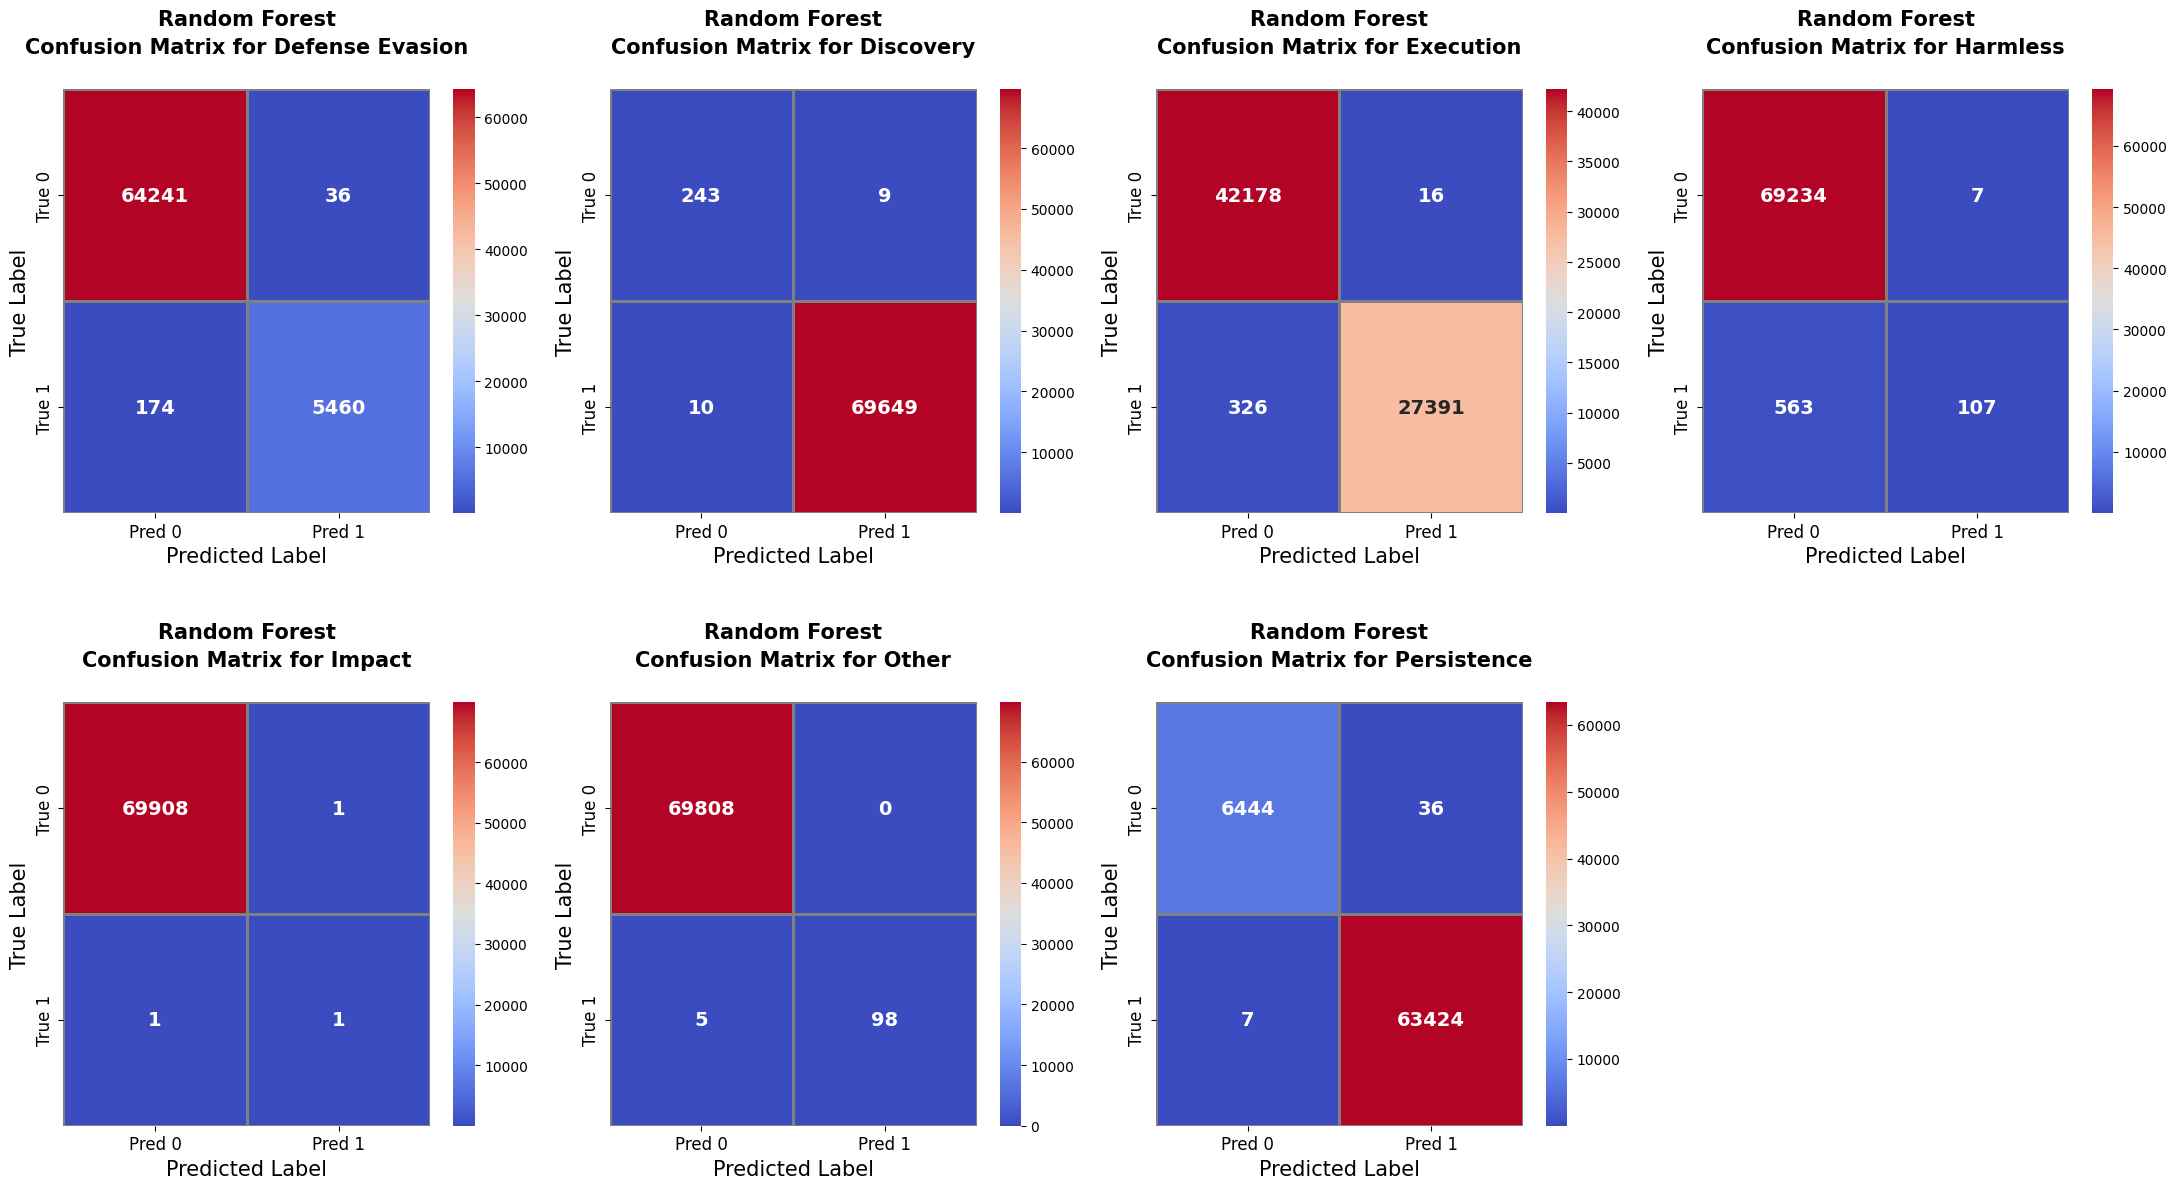
\includegraphics[width=0.77\textwidth]{../figures/plots/section2/Random_Forest_normalized_confusion_matrix_test.png}
                    \caption{Random Forest Confusion Matrices}
                    \label{fig:rf_cm_base}
                \end{minipage}%
            \end{minipage}

            \vspace{0.5cm}  % Add some vertical spacing between rows
            
            % Middle row  
            \begin{minipage}{\textwidth}
                % Middle-left (Train)
                \begin{minipage}[c]{0.48\textwidth}
                    \centering
                    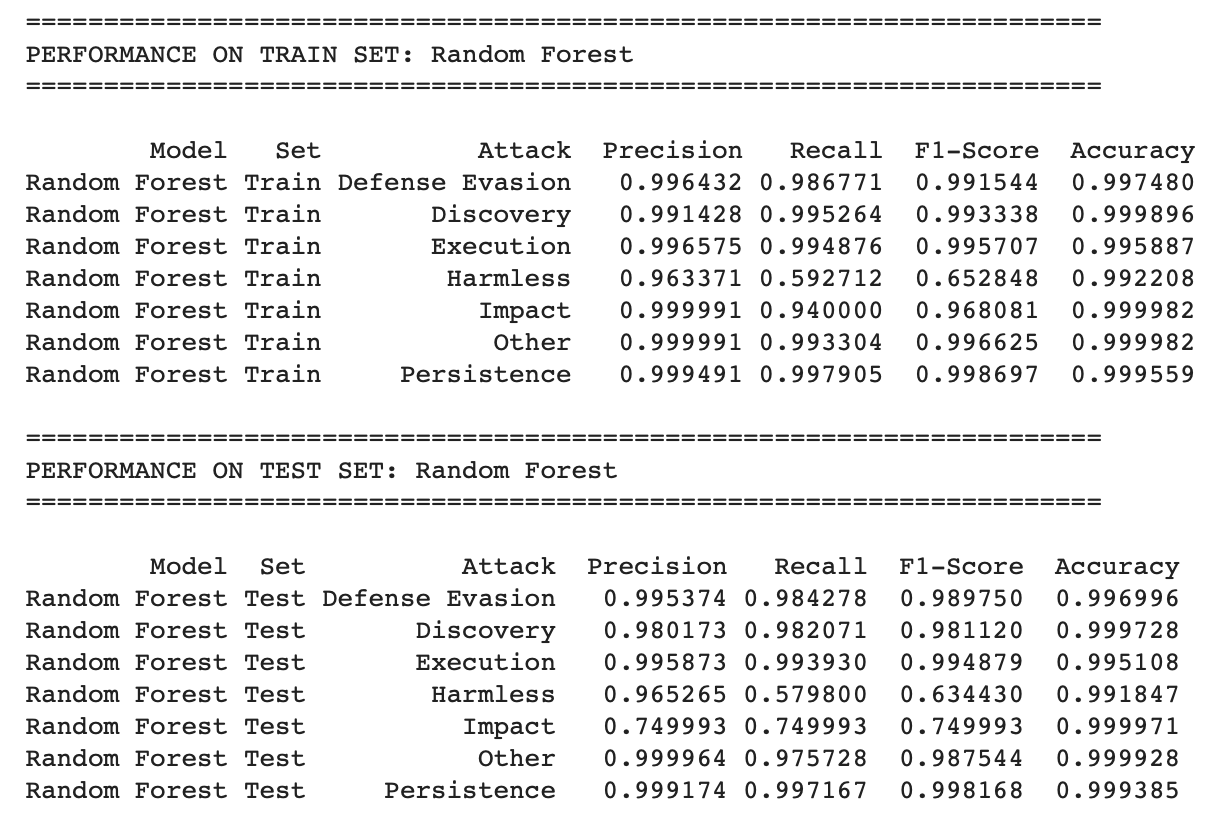
\includegraphics[width=0.9\textwidth]{../figures/plots/section2/Random_Forest_evaluation_metrics.png}
                    \caption{Random Forest Evaluation Metrics}
                    \label{fig:rf_em_base}
                \end{minipage}%
                \hfill%
                % Middle-right (Train)
                \begin{minipage}[c]{0.48\textwidth}
                    \centering
                    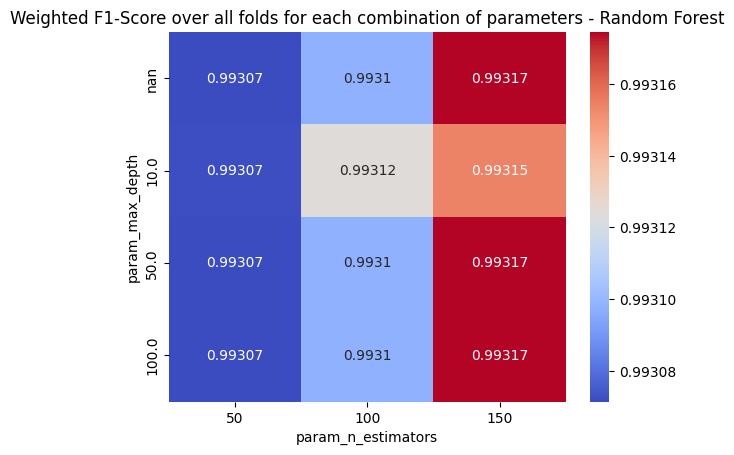
\includegraphics[width=0.7\textwidth]{../figures/plots/section2/weighted_f1_score_for_each_combination_of_parameters_random_forest.png}
                    \caption{Random Forest Weighted F1 Scores}
                    \label{fig:rf_f1_tuning}
                \end{minipage}
            \end{minipage}
            
            \vspace{0.5cm}  % Add some vertical spacing between rows

            % Bottom row
            \begin{minipage}{\textwidth}
                % Bottom-left (Test)
                \begin{minipage}[t]{0.48\textwidth}
                    \centering
                    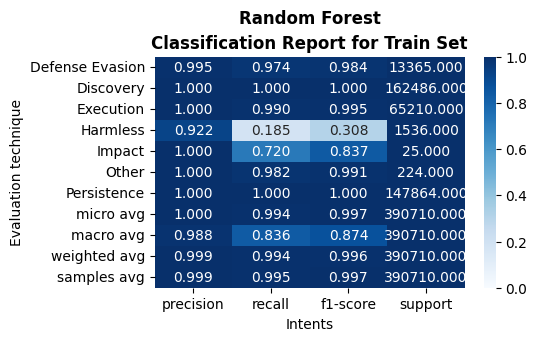
\includegraphics[width=0.9\textwidth]{../figures/plots/section2/Random_Forest_classification_report_for_Train_set.png}
                    \caption{Random Forest Classification Report Train Set}
                    \label{fig:rf_cm_train}
                \end{minipage}%
                \hfill%
                % Bottom-right (Test)
                \begin{minipage}[t]{0.48\textwidth}
                    \centering
                    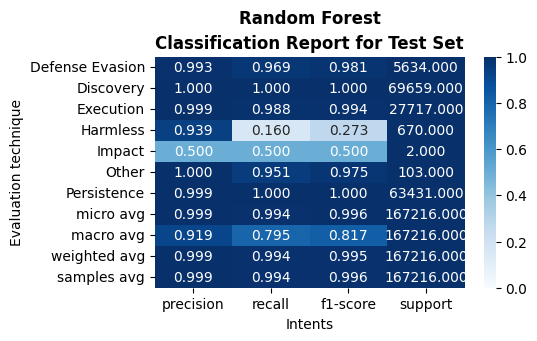
\includegraphics[width=0.9\textwidth]{../figures/plots/section2/Random_Forest_classification_report_for_Test_set.png}
                    \caption{Random Forest Classification Report Test Set}
                    \label{fig:rf_cm_test}
                \end{minipage}  
            
            \end{minipage}
            
        \end{figure}
            
        \clearpage
    
        % SVM
        
        \begin{figure}[H]
        
            \centering
            
            % Top row
            \begin{minipage}{\textwidth}
                \centering
                \begin{minipage}[c]{\textwidth}
                    \centering
                    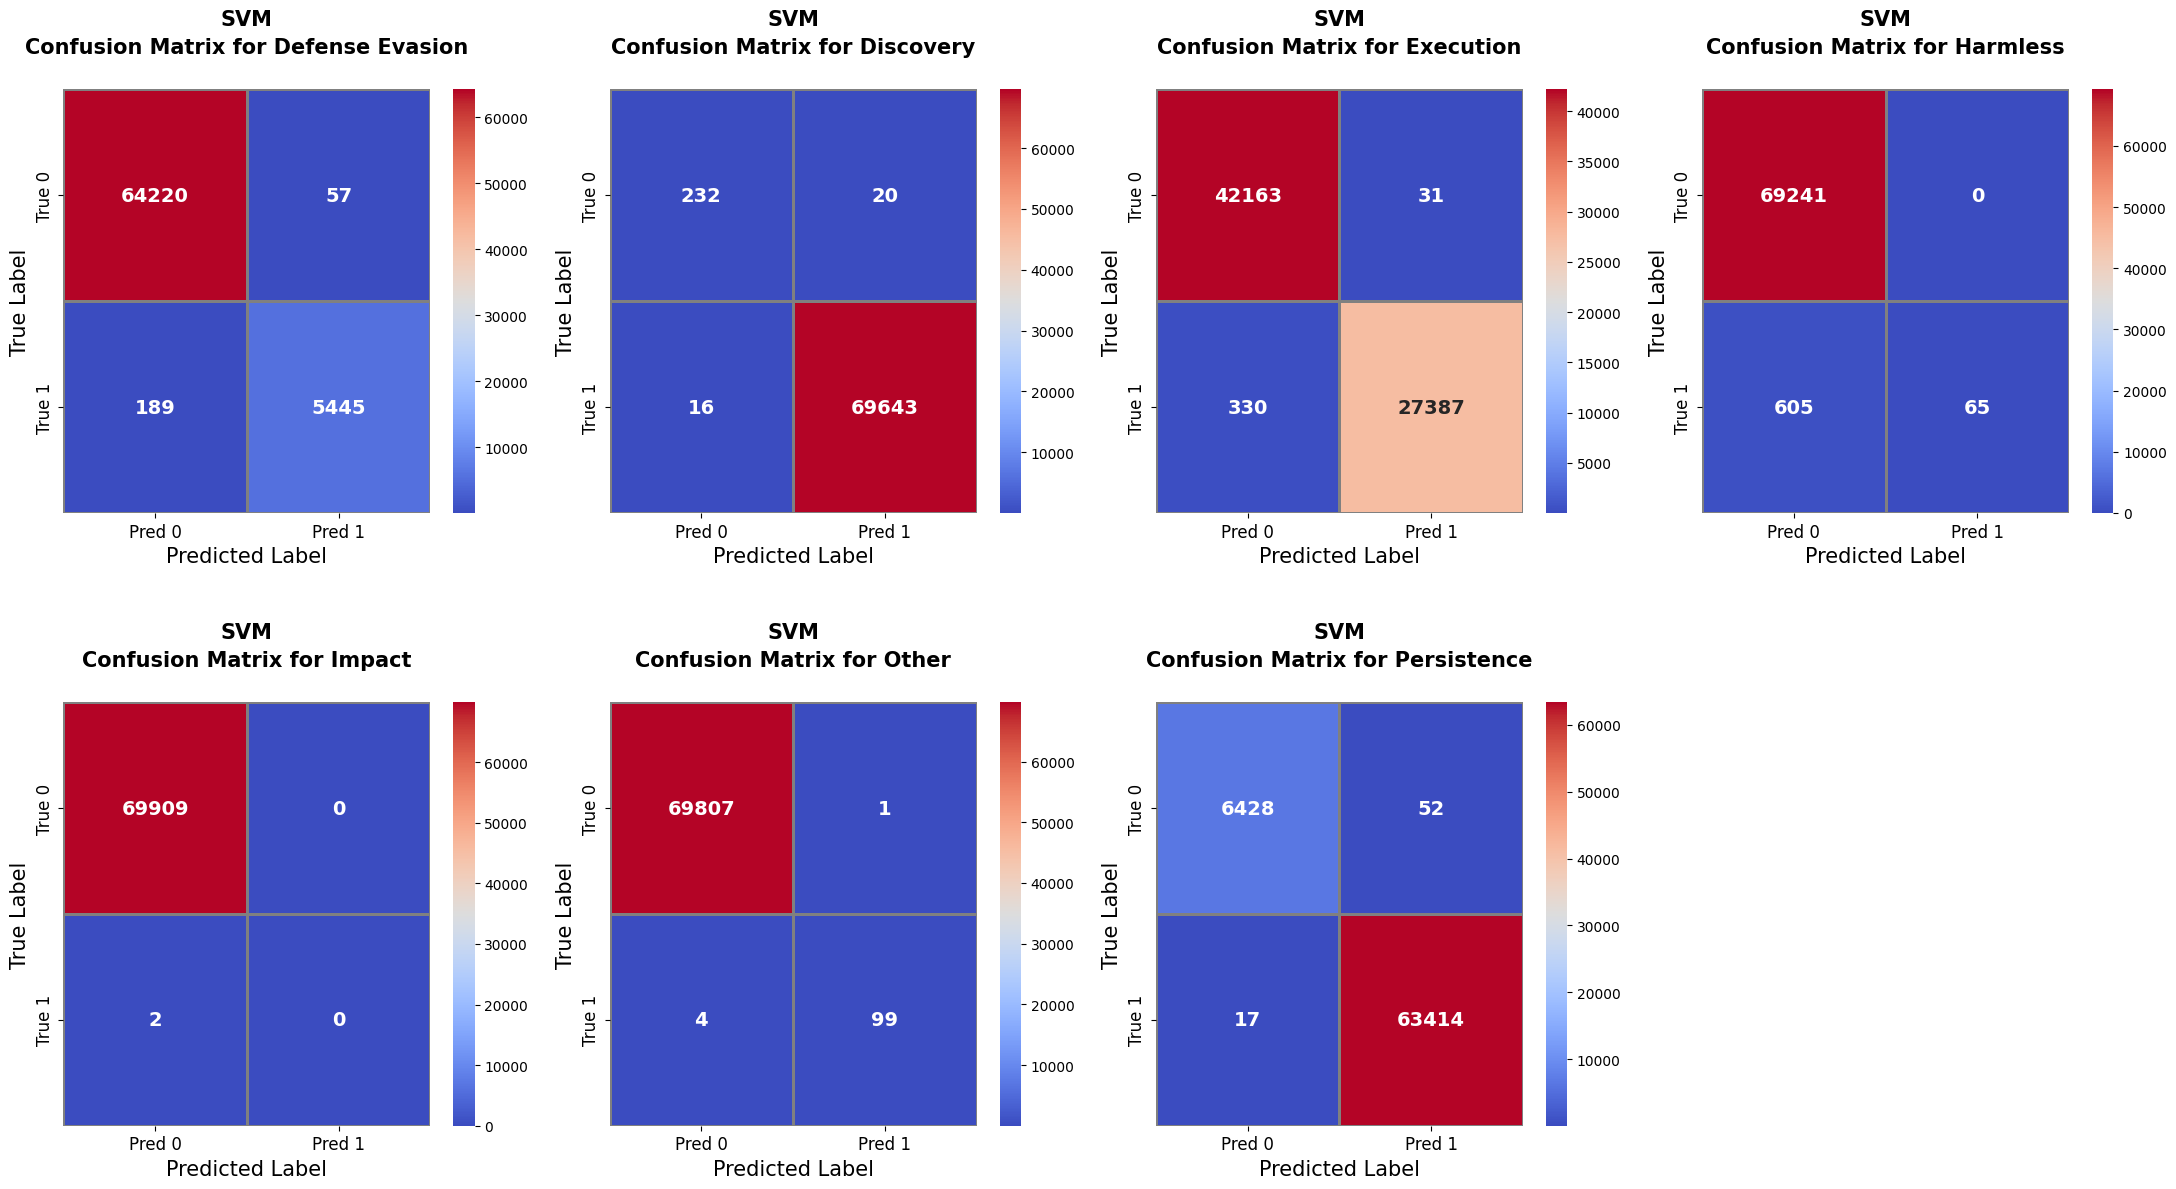
\includegraphics[width=0.77\textwidth]{../figures/plots/section2/SVM_normalized_confusion_matrix_test.png}
                    \caption{SVM Confusion Matrices}
                    \label{fig:svm_cm_base}
                \end{minipage}%
            \end{minipage}

            \vspace{0.5cm}  % Add some vertical spacing between rows
            
            % Middle row  
            \begin{minipage}{\textwidth}
                % Middle-left (Train)
                \begin{minipage}[c]{0.48\textwidth}
                    \centering
                    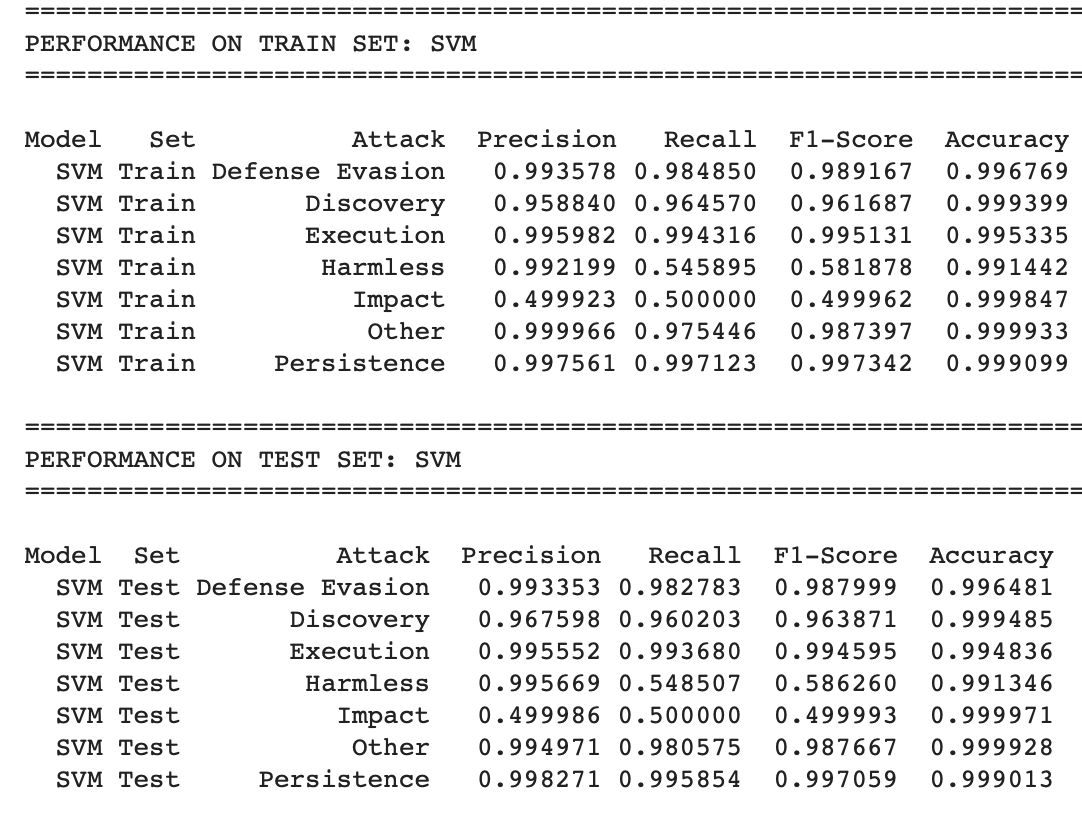
\includegraphics[width=0.8\textwidth]{../figures/plots/section2/SVM_evaluation_metrics.png}
                    \caption{SVM Evaluation Metrics}
                    \label{fig:svm_em_base}
                \end{minipage}%
                \hfill%
                % Middle-right (Train)
                \begin{minipage}[c]{0.48\textwidth}
                    \centering
                    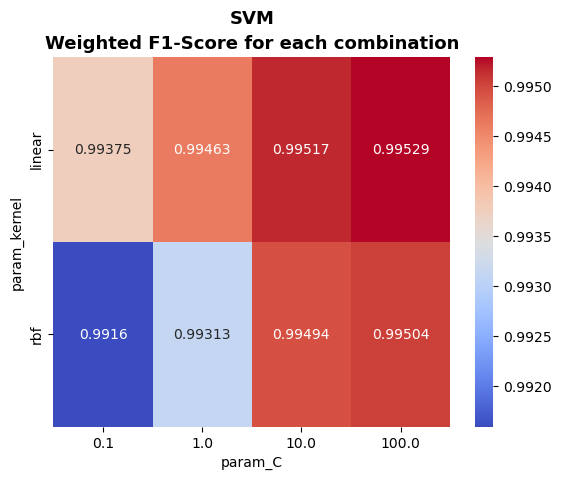
\includegraphics[width=0.7\textwidth]{../figures/plots/section2/weighted_f1_score_for_each_combination_of_parameters_svm.png}
                    \caption{SVM Weighted F1 Scores}
                    \label{fig:svm_f1_tuning}
                \end{minipage}
            \end{minipage}
            
            \vspace{0.5cm}  % Add some vertical spacing between rows

            % Bottom row
            \begin{minipage}{\textwidth}
                % Bottom-left (Test)
                \begin{minipage}[t]{0.48\textwidth}
                    \centering
                    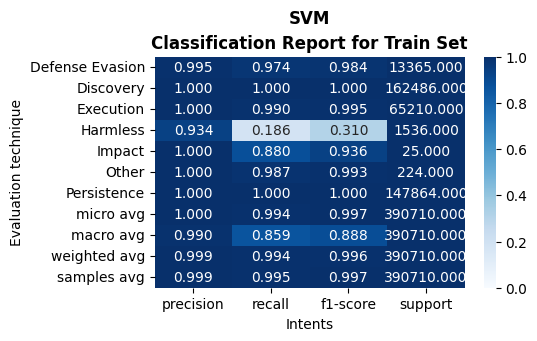
\includegraphics[width=0.9\textwidth]{../figures/plots/section2/SVM_classification_report_for_Train_set.png}
                    \caption{SVM Classification Report Train Set}
                    \label{fig:svm_cm_train}
                \end{minipage}%
                \hfill%
                % Bottom-right (Test)
                \begin{minipage}[t]{0.48\textwidth}
                    \centering
                    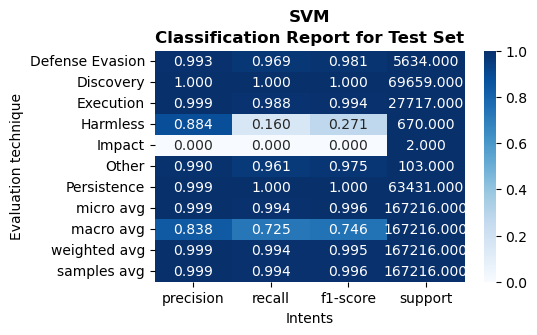
\includegraphics[width=0.9\textwidth]{../figures/plots/section2/SVM_classification_report_for_Test_set.png}
                    \caption{SVM Classification Report Test Set}
                    \label{fig:svm_cm_test}
                \end{minipage}  
            
            \end{minipage}
            
        \end{figure}
